
\documentclass[conference, letterpaper]{IEEEtran}

\usepackage{listings}
\usepackage{minted}
\usemintedstyle{bw}

\hyphenation{op-tical net-works semi-conduc-tor}

% *** GRAPHICS RELATED PACKAGES ***
\ifCLASSINFOpdf
   \usepackage[pdftex]{graphicx}
   \graphicspath{ {figures/} }
\else
\fi

% *** MATH PACKAGES ***
\usepackage[cmex10]{amsmath}
\usepackage{color}
\usepackage{fancyhdr}
\usepackage[caption=false,font=footnotesize]{subfig}

\renewcommand{\thispagestyle}[2]{} 

\newcommand{\padlisting} {
    \begin{minted}{text}
    \end{minted}
}

\fancypagestyle{plain}{
        \fancyhead{}
        \fancyhead[C]{first page center header}
        \fancyfoot{}
        \fancyfoot[C]{first page center footer}
}
\pagestyle{fancy}

\headheight 31.99992pt
\footskip 20pt

\rhead{}

\setcounter{page}{1}

\fancyhead[R]{\textit{RIT Computer Science ~\textbullet~ Capstone Report ~\textbullet~ 2171}}
\renewcommand{\headrulewidth}{0pt}

%Footer
\fancyfoot[C]{Rochester Institute of Technology}
\renewcommand{\footrulewidth}{0.5pt}
\fancyfoot[R]{\thepage \  $|$ P a g e }

\begin{document}

\title{Using Transactional Events in Haskell in the Impelementation of Message Broker Middleware}

\author{\IEEEauthorblockN{Christopher R. Wicks}
\IEEEauthorblockA{Department of Computer Science\\Golisano College of Computing and Information Sciences\\
Rochester Institute of Technology\\
Rochester, NY 14586\\
cw9887@cs.rit.edu}}

\maketitle

\begin{abstract}
Transactional events are used in the  implementation of message broker middleware. In particular, STOMP 
(Simple Text Oriented Messaging Protocol) client APIs, shared libraries, and a message broker are implemented 
utilizing an experimental transactional events library built on Concurrent Haskell.
\end{abstract}

\begin{IEEEkeywords}
Transactional Events, Concurrency, Haskell, Functional Programming, Monad, Message Broker, 
Message Oriented Middleware, STOMP
\end{IEEEkeywords}

\IEEEpeerreviewmaketitle

\section{Introduction}
Transactional events are a relatively recent concurrency abstraction in the functional programming
paradigm. They are a high-level abstraction that combine the first-class synchronous message-passing events
of Concurrent ML (CML) with all-or-nothing transactions \cite{te:original}. Their inception draws
inspiration from CML, Concurrent Haskell, and Software Transactional Memory (STM) Haskell. There currently 
exist implementations as language extensions for both Haskell \cite{te:original} and ML \cite{te:ml}.

Transactional events are primarily motivated by the need for better abstractions in the development of 
concurrent programs. The non-deterministic execution order of concurrent programs makes them inherently
difficult to reason about. Transactional events help to ease some of the pain by allowing for inter-thread
communications to be composed of modular events in the form of transactions.

STOMP, the Simple (or Streaming) Text Oriented Message Protocol, is a text-based message passing protocol from the same school of design as HTTP.
\cite{stomp:spec}. It is designed so that applications in a distributed software system can communicate easily (from the 
perspective of an application developer) over a network.

``Every programming model needs three things: a semantics, an implementation, and useful idioms" 
\cite{te:idioms}. The semantics and the implementation have been provided in the work laid out in \cite{te:original}.
In this work, we explore the use of transactional events in the implementation and API design of a
collection of software tools and applications utilizing the STOMP protocol. We implement a client 
API, an command-line client application, a message broker (server), and shared libraries utilizing 
Transactional Events Haskell (TE Haskell). In particular, we identify useful idioms, patterns,
and interesting use cases for transactional events as a programming model.

\section{The STOMP Protocol}

STOMP is used primarily in the domain of message-oriented middleware. In these scenarios, many clients
communicate with one or more servers, or message brokers, via some protocol. The message brokers then contain the necessary routing and transformation logic to pass that information on to other interested clients who may or may not be using the same protocol.

STOMP is designed to be a very simple and easy to use protocol. The STOMP 1.2 specification supports 11 different client frames and 4 different server frames. One particularly interesting aspect of the protocol for the purposes of this work is the support of client-initiated transactions.

The STOMP protocol is \textit{text-based}, with the command and header portion of the frames encoded using UTF-8. The frame body, if present, may be encoded arbitrarily, and may even contain binary data. A frame consists of a command, 0 or more headers followed bye a blank line, and a body which may be empty. A frame must always be terminated by a null octet (\^{}@):

\begin{minted}{text}
    COMMAND
    header1:value1
    header2:value2

    Message body^@
\end{minted}

\subsection{Client Frame Commands}

The CONNECT and STOMP frames are equivalent in version 1.2 of the protocol; STOMP is preferred, but CONNECT is preserved for backwards compatibility. These frames allow the client to initiate a connection to a STOMP broker. The DISCONNECT frame allows a client to gracefully disconnect from a session with a STOMP broker. The SUBSCRIBE and UNSUBSCRIBE client frames allow a client to register and deregister their willingness to receive messages from a given destination. The ACK and NACK frames allow a client to either acknowledge of disacknowledge the processing of a received message. The BEGIN, COMMIT, and ABORT frames, respectively, allow the client to begin, commit, or abort a named transaction.

\subsection{Server Frame Commands}

The server only has 4 frames that it may send to a client. The CONNECTED frame acknowledges a successful connection request from the client and contains the results of both protocol negotiations (the highest protocol version supported by both client and server) and heartbeat negotiations. The MESSAGE frame contains message data from a registered destination. The RECEIPT frame contains a receipt for a frame sent by the client in which a receipt was requested via a special header. The ERROR frame indicates a protocol or processing error. After sending an ERROR frame, the protocol dictates the the server close the connection immediately.

\subsection{Transactions}
STOMP supports client-initated named transactions, in which it is requested that all messages sent as part of a given transaction are processed atomically by the server. STOMP brokers support the ability for a single client to have multiple ongoing transactions at any given time (the frames need not be sent atomically, or even successively), with the server keeping track of the state. Only SEND, ACK, and NACK frames may be part of a transaction, with the BEGIN, COMMIT, and ABORT frames managing the control. Whether or not a message is part of a transaction, or the specification of which transaction a control frame is referring to, is handled using the transaction frame header. An example of a SEND frame that is to be processed as part of the named transaction \textit{tx1} is given:

\begin{minted}{text}
    SEND
    destination:q1
    content-type:text/plain
    content-length:13
    transaction:tx1

    Hello, world!^@
\end{minted}

\subsection{Heart-beating}
STOMP supports bidirectional heart-beats between the client and server. If heart-beats are expected, the sender must send either a frame or a heart-beat at least once every \textit{n} milliseconds. A heart-beat is comprised simply of an end-of-line (EOL) character. If a longer interval transpires without having received any data, the receiver may consider the connection lost and close it. The client will send, in the STOMP or CONNECT frame, the minimum rate of heart-beats that it is able to both send and receive, if any. The server then compares those values to its own capabilities, and chooses the longest interval (or, if either client or server does not wish to send or receive heartbeats, 0 is chosen). An example of the STOMP frame is given:

\begin{minted}{text}
    STOMP
    accept-version:1.0,1.1,1.2
    host:wicks.com
    heart-beat:4000,0
    
    ^@
\end{minted}

The first value in the heart-beat header indicates that the client is able to send heart-beats as quickly as once every 4000 milliseconds.  The second value in the heart-beat header indicates that the client does not wish to receive heart-beats from the server. If, for example, the server to which it is connecting only wishes to receive heart-beats every 10000 milliseconds, the corresponding CONNECTED acknowledgement would look as follows:

\begin{minted}{text}
    CONNECTED
    accept-version:1.2
    heart-beat:0,10000
\end{minted}

Note that the value of zero indicates that the server will not be sending heart-beats, even if it did support such, as the client has requested not to receive them. The value of 10000 indicates that based on the client's capabilities and its own expectations that it expects to receive either a heartbeat every 10000 milliseconds (the maximum value between the client's send rate and its own receive rate). Also note that heart-beating capabilities are dictated by the client. A server is free to reject a client if its heart-beating capabilities are not up to its minimum requirements, but this is an implementation detail and is not dictated by the protocol.

\section{Transactional Events}
\setminted{fontsize=\scriptsize,baselinestretch=1}

The basic transactional events interface given by Fluet and Donnelly \cite{te:original} is provided in Figure \ref{monadcode} for ease of refernece.

\begin{figure}[h]
    \begin{minted} {haskell}
        data Evt a

        sync :: Evt a -> IO a
        thenEvt :: Evt a -> (a -> Evt b) -> Evt b
        alwaysEvt :: a -> Evt a
        chooseEvt :: Evt a -> Evt a -> Evt a
        neverEvt :: Evt a

        instance Monad Evt where
           (>>=) = thenEvt
           return = alwaysEvt

        instance MonadPlus Evt where
            mplus = chooseEvt
            mzero = neverEvt

        data SChan a -- Synchronous channels
        newSChan :: Evt (SChan a)
        sendEvt :: SChan a -> a -> Evt ()
        recvEvt :: SChan a -> Evt a
    \end{minted}
    \caption{The Evt Monad}
    \label{monadcode}
    \centering
\end{figure}

This interface is used by composing events using the provided event combinators: \textit{thenEvt, alwaysEvt, chooseEvt}, and \textit{neverEvt}. We then use the \textit{sync} function to synchronize on an event. Said synchronization blocks until the event is able to complete, and the result is returned wrapped in the \textit{IO} monadic context. The synchronous channels allow us to create event channels that can be used to pass messages between concurrently executing threads. There are additional combinators, \textit{sendEvt} and \textit{recvEvt}, that allow the composition of events that pass messages between multiple threads. Any send on a synchronous channel must be matched with a corresponding receive in another thread on the same channel in order to be able to synchronize. A simple "Hello, world!" program using transactional events can be constructed as demonstrated in Figure \ref{helloworld}.

\begin{figure}[h]
    \begin{minted} {haskell}
      import Control.Concurrent
      import Control.Concurrent.TxEvent

      main :: IO ()
      main = do
        channel <- sync newSChan
        forkIO $ sync (sendEvt channel "Hello, world!")
        s <- sync $ recvEvt channel
        putStrLn s
    \end{minted}
    \caption{"Hello, World!" Using Transactional Events}
    \centering
    \label{helloworld}
\end{figure}

This program first synchronizes on the creation of a new synchronous communications channel, forks off a thread that sends a String on the channel, and then blocks until it receives a String on the same channel, finally displaying it on the standard output. Note that if we were to attempt to write this program without forking off the send to take place in a new thread, the initial synchronization on \textit{sendEvt} would block indefinitely.

One of the primary attributes of transactional events that makes them an attractive tool for concurrent programming, and the one that sets the idiom apart from the similar message-passing style found in CML, is the fact that they are easily composable due to their monadic structure. As seen here, in the Haskell implementation the \textit{Evt} typeclass is a subclass of both \textit{Monad} and \textit{MonadPlus}. This allows for easy sequencing of events utilizing Haskell's \textit{do} notation, as the monadic bind is implemented as the \textit{thenEvt} combinator. Using this combinator, one can compose an event comprised of smaller events that must be able to complete in sequence. If any individual event in the composite is unable to complete, the entire event ``fizzles" without any side-effects that are observable by the rest of the system, providing a transactional guarantee for event synchronization.

The interface also provides a non-deterministic choice combinator in the form of \textit{chooseEvt}. This allows an event to synchronize on whichever of the two events it is able to synchronize on first, effectively aborting the computations performed in the event that is not chosen. Note that \textit{neverEvt} is the event that can never be synchronized upon. Hence, sequencing a \textit{neverEvt} using the monadic bind is an effective abort. Likewise, the \textit{chooseEvt}, as it cannot choose an event that will not successfully complete, will never synchronize on the \textit{neverEvt}.

Using this interface, one can easily compose sophisticated computational event structures that allow for inter-thread communication but guarantee that irrevocable side effects can not take place during event synchronization (hence the "all-or-nothing" transactional claim). Indeed, transactional events are shown to be strictly more expressive than either STM Haskell and CML in \cite{te:original}. The authors provide encodings for both idioms using transactional events. The then demonstrate that one can express computations that are not possible in either, such as \textit{n}-way synchronization between threads.

% \section{Project Goals}

% The primary goal of this project was to implement a message broker, client software, and APIs for the STOMP protocol using Haskell with transactional events. [needs more, but what?]

\section{Library Design \& Usage}

\subsection{Stomp.Frames}

The initial challenge in implementing the shared libraries was in determining exactly how STOMP frames should be represented, and how they would be passed back-and-forth over a TCP connection. The Frame data type was designed as shown in Figure \ref{frame}, and was designed such that it can be easily parsed and constructed piecemeal while reading bytes from a socket handle.

\begin{figure}[h]
    \begin{minted} {haskell}
    -- |A HeaderName is a type synonym for String, and 
    -- is one component of a Header
    type HeaderName     =   String

    -- |A HeaderValue is a type synonym for String, and 
    -- is one component of a Header
    type HeaderValue    =   String

    -- |A Header contains a name and a value for a 
    -- STOMP header
    data Header         =   Header HeaderName HeaderValue

    -- |A Headers is a recursive, list-like data structure 
    -- representing the set of Headers for a STOMP frame
    data Headers        =   Some Header Headers | EndOfHeaders

    -- |A Body represents the body of a STOMP frame. It
    -- is either empty or consists of a single ByteString.
    data Body           =   EmptyBody | Body ByteString

    -- |A Command represents the command portion of 
    -- a STOMP Frame.
    data Command        =   SEND |
                            SUBSCRIBE |
                            UNSUBSCRIBE |
                            BEGIN |
                            COMMIT |
                            ABORT |
                            ACK |
                            NACK |
                            DISCONNECT |
                            CONNECT |
                            STOMP |
                            CONNECTED |
                            MESSAGE |
                            RECEIPT |
                            ERROR deriving Show

    -- |An abstract data type representing a STOMP Frame.
    -- It consists of a Command, Headers, and Body.
    data Frame          =   Frame Command Headers Body
    \end{minted}
    \caption{The Frame Data Type}
    \label{frame}
    \centering
\end{figure}

The definition for the Frame datatype is contained within the \textit{Stomp.Frames} module of the \textit{tehstomp-lib} library package. Additionally, that module exports a plethora of utility functions for constructing, manipulating, and extracting information from Frames, including straightforward constructions for all of the commands with their required headers. Utilizing this interface it is simple for clients of the library to construct any possible STOMP frame.

\subsection{Stomp.Frames.IO}

Another module provided by the \textit{tehstomp-lib} package is called \textit{Stomp.Frames.IO}. This module encapsulates error-handling IO operations on Handles that are expected to be receiving STOMP frames. In most cases, this will be a Handle to a TCP socket connection in a STOMP client or broker, although any producer or consumer of STOMP frames could be handled using the library. The FrameHandler datatype utilizes transactional events to provide multiple asynchronous readers and writers with synchronous access to the underlying Handle as Frames are read and written. To achieve this, the datatype houses two synchronous channels (SChans). Clients obtain a FrameHandler by using the \textit{initFrameHandler} function. We obtain two synchronous channels, and then fork off looping threads that handle their processing (see Figure \ref{framehandler}).

\begin{figure}[h]
    \begin{minted} {haskell}
    -- |Given a resource Handle, initialize a FrameHandler
    -- and return it in an IO context.
    initFrameHandler :: Handle -> IO FrameHandler
    initFrameHandler handle = do
        writeChan <- sync newSChan
        readChan  <- sync newSChan
        forkIO $ writeLoop handle 0 writeChan
        forkIO $ readLoop handle readChan
        return $ FrameHandler handle writeChan readChan

    data FrameEvt = NewFrame Frame |
                    ParseError String |
                    Heartbeat |
                    GotEof |
                    TimedOut

    parseFrame :: Handle -> IO FrameEvt

    frameReaderLoop :: Handle -> SChan FrameEvt -> IO ()
    frameReaderLoop handle readChan = do
        evt <- parseFrame handle
        sync $ sendEvt readChan evt
        case evt of 
            NewFrame _ -> frameReaderLoop handle readChan
            Heartbeat  -> frameReaderLoop handle readChan
            -- Terminate the loop in the error case
            otherwise  -> return ()

    -- |Get the next FrameEvt from the FrameHandler and
    -- return it in an Evt context.
    getEvt :: FrameHandler -> Evt FrameEvt
    getEvt (FrameHandler _ _ readChannel _ _) = 
        recvEvt readChannel
    \end{minted}
    \centering
    \caption{The FrameHandler}
    \label{framehandler}
\end{figure}

The \textit{frameReaderLoop} function shown above loops waiting for input on a handle (the \textit{parseFrame} function), and then attempts to synchronize on its \textit{SChan}. When a client synchronizes on the \textit{getEvt} function, the synchronization occurs, the FrameEvt is returned in an IO context, and the next frame is parsed. The API takes a two-tiered approach. The bare Evt functions are exposed, along with functions that abstract the event synchronization away from the client (an analogous \textit{get} function is provided as well). This offers some flexibility in the construction of applications using these events.

For readers that are expecting heart-beats, we offer an additional function that times out if no data is received on the Handle, shown in figure \ref{recv-heartbeat}.

\begin{figure}[h]
    \begin{minted} {haskell}
    getEvtWithTimeOut :: FrameHandler -> Int -> Evt FrameEvt
    getEvtWithTimeOut (FrameHandler _ _ readChannel) n = 
        if n < 1 then
            recvEvt readChannel
        else
            (recvEvt readChannel) `chooseEvt` 
                (timeOutEvt n `thenEvt` 
                    (\_ -> alwaysEvt TimedOut))
    \end{minted}
    \caption{Heart-beat Management for Receivers}
    \label{recv-heartbeat}
\end{figure}

The \textit{timeOutEvt} is part of the extended \textit{TxEvents} library detailed in \cite{te:original}. It is an event that becomes available for synchronization after a given number of microseconds has transpired. In this particular case, the \textit{timeOutEvt} is sequenced with an \textit{alwaysEvt} that will always return \textit{TimedOut}; note that the \textit{timeOutEvt} simply returns the unit value, and this particular function needs to return a \textit{TimeOutEvt}. This necessitates the usage of the \textit{thenEvt} sequencing combinator as shown above. Without the availability of this combinator, returning default values or specifying alternative control flows for timeouts in event processing would require much more complex logic. As it is, we can specify the ``next step" to take after a timeout simply and logically. When a client synchronizes on the \textit{getEvtWithTimeOut} event, if we have to wait longer than the given time allotment to receive an event on the read channel, the second choice is taken, and \textit{TimedOut} is returned to the client.

The \textit{FrameHandler} abstraction also provides functionality for \textit{automatically} generating heartbeats if so needed (see Figure \ref{send-heartbeat}). This allows the client of this library, be it a client or a server application, to simply ``set and forget" once initial negotiations have transpired.

\begin{figure}[h]
    \begin{minted} {haskell}
    data SendEvt  = SendFrame Frame |
                    UpdateHeartbeat Int |
                    DoHeartbeat

    -- |Puts the given Frame into the FrameHandler in an Evt context.
    putEvt :: Frame -> FrameHandler -> Evt ()
    putEvt frame (FrameHandler _ writeChan _ _ _) = 
        sendEvt writeChan $ SendFrame frame

    -- |Update the rate at which this FrameHandler sends 
    -- heart-beats. A rate of 0 or less means that no 
    -- heart-beats will be transmitted. Otherwise, we 
    -- will send one heart-beat every n microseconds.
    updateHeartbeat :: FrameHandler -> Int -> IO ()
    updateHeartbeat (FrameHandler _ writeChan _ _ _) n = 
        sync $ sendEvt writeChan (UpdateHeartbeat n)

    frameWriterLoop :: Handle -> Int -> SChan SendEvt -> IO ()
    frameWriterLoop handle freq writeChan = do
        update <- if freq < 1 
            then sync $ recvEvt writeChan
            else sync $ (recvEvt writeChan) `chooseEvt` 
                (timeOutEvt freq `thenEvt` 
                  (\_ -> alwaysEvt DoHeartbeat))
        case update of
            SendFrame frame -> do
                hPut handle $ frameToBytes frame
                frameWriterLoop handle freq writeChan
            UpdateHeartbeat freq' -> do
                hPut handle $ UTF.fromString "\n"
                frameWriterLoop handle freq' writeChan
            DoHeartbeat       -> do
                hPut handle $ UTF.fromString "\n"
                frameWriterLoop handle freq writeChan
    \end{minted}
    \centering
    \caption{Heart-beat Management for Senders}
    \label{send-heartbeat}
\end{figure}

Since the protocol dictates that the sender delivers either a frame or a heartbeat at least once per interval, and whether or not a sender is going to send a frame at some point during that interval is non-deterministic, we construct the event using the \textit{chooseEvt} combinator. This event will either send a frame if one is provided within the interval, or send a heartbeat after said interval has transpired without receiving any frames to transmit. We also provide a means for updating the heartbeat after the loop has been initiated. The reasoning for this is that it is likely that a client or server will want to use the FrameHandler in setting up heart-beating and protocol negotiations, so it will need to be initialized prior to the final frequency determination. This allows for those initial negotiations to take place and the heart-beating mechanism to be kicked off after the fact if necessary.

\subsection{Stomp.Frames.IO.Router}

\textit{[Note to the early reader of this report: there are aspects of this system that are still not quite complete, but will be for the final project]}

One can envision a client application in which multiple system components are interested in the different types of frames that are received from the server. As part of the \textit{tehstomp-lib} library, we provide a client-centric (in that it would be not suitable for use in a server implementation) event management system, wrapping a \textit{FrameHandler}, that routes frames to registered listeners. The exported API is given in Figure \ref{framerouter}.

\begin{figure}[h]
    \begin{minted} {haskell}
    data RequestHandler = RequestHandler (SChan Update)

    initFrameRouter :: 
      FrameHandler -> 
      IO RequestHandler

    -- |Request a dedicated channel on which to receive
    -- CONNECTED and RECEIPT Frames
    requestResponseEvents :: 
      RequestHandler -> 
      IO (SChan FrameEvt)

    -- |Request a dedicated channel on which to receive
    -- MESSAGE frames for the given subscription ID
    requestSubscriptionEvents :: 
      RequestHandler -> 
      String -> IO (SChan FrameEvt)

    -- |Request a dedicated channel on which to receive
    -- heart-beats
    requestHeartbeatEvents :: 
      RequestHandler -> 
      IO (SChan FrameEvt)

    requestErrorEvents :: 
      RequestHandler -> 
      IO (SChan FrameEvt)
    \end{minted}
    \centering
    \caption{The FrameRouter API}
    \label{framerouter}
\end{figure}

Once the \textit{RequestHandler} has been initialized with a \textit{FrameHandler}, interested system components can use it to obtain dedicated event channels. The \textit{FrameRouter} maintains lists of those channels, and when a relevant \textit{FrameEvt} is received, it is broadcast to all registered listeners. Clients can register for frames that are sent to individual subscriptions (MESSAGE), frames that are sent as responses (CONNECTED, RECEIPT), or ERROR frames. They can also request to receive heart-beats. Per-frame processing for each registered channel is handled on a separate thread, so that no individual registered component is able to hold up processing for any of the other registered components.

\subsection{Additional Modules}
There are a few additional modules exported by the library that do not have to do with STOMP directly, but are useful nonetheless and are mentioned here in brief. The \textit{Stomp.TLogger} module implements a transactional ``logger", similar but simpler in concept and design to that of the \textit{FrameHandler}. The \textit{Stomp.Increment} module implements a stateful incrementer, and was motivated by the need for an unbounded value for generating unique message identifiers across the lifetime of a server instance. In earlier phases of the implementation, the application was using the \textit{Data.Unique} package for generating message identifiers, but the values produced by such hash out to a bounded \textit{Int} datatype. In principle, depending on the compiler, the upper bound on the values produced could be as low as \begin{math}2^{28}\end{math} \cite{data:int}, which is likely to be insufficient for a long-running, high-activity server. In practice, most implementations place a much higher upper bound on the \textit{Int} type, but the \textit{Integer} type is unbounded in Haskell, making it a more attractive candidate for such identifiers.
\section{Server Application Design \& Usage}

Two applications were developed using transactional events, along with the \textit{tehstomp-lib} libraries developed as part of this project: a basic command-line STOMP client, and a STOMP message broker.

\subsection{The STOMP Broker}

At the core of the STOMP broker is a looping function over an open socket. The function loops as connections are received, and forks off a new thread to negotiate each incoming connection request. 

\begin{figure}[h]
    \begin{minted} {haskell}
    socketLoop :: 
        Socket -> 
        Logger -> 
        SubscriptionManager ->
        Incrementer -> 
        IO ()
    socketLoop sock console subManager inc = do
        (uSock, _) <- accept sock
        addr <- getPeerName uSock
        log console $ "New connection received from " 
            ++ (show addr)
        handle <- socketToHandle uSock ReadWriteMode
        hSetBuffering handle NoBuffering
        frameHandler <- initFrameHandler handle
        forkIO $ negotiateConnection frameHandler 
            (addTransform (appendTransform 
                ("[" ++ show addr ++ "]")) console)
                    subManager inc
        socketLoop sock console subManager inc
    \end{minted}
    \centering
    \caption{STOMP Broker Socket Loop}
\end{figure}

If protocol negotiations are successful, the handle remains open, and the thread loops waiting for frames and heartbeats from the client until the client disconnects. The connection data for a given client is encapsulated in the \textit{Connection} datatype:


\begin{figure}[h]
    \begin{minted} {haskell}
    -- |Encapsulation of a single client's connection data
    data Connection      = Connection 
                           ClientId 
                           FrameHandler 
                           ClientTransactionManager 
                           Int
    \end{minted}
    \centering
    \caption{Client Connection Data}
    \label{connectiondata}
\end{figure}


The \textit{ClientId} is a unique identifier for the client that is to be used in the \textit{SubscriptionManager}. The server has a single stateful \textit{Incrementer} that it uses to generate unique client identifiers. The \textit{FrameHandler} is constructed using the \textit{Handle} obtained from the socket connection. The \textit{ClientTransactionManager} is a dedicated transaction manager for that client, and the \textit{Int} is the frequency with which heart-beats are expected to be received from the client. The \textit{ClientTransactionManager} contains a stateful loop that is maintained per-client, as the rest of the system doesn't need to be aware of pending client transactions. The \textit{ClientTransactionManager} will be discussed in more detail in the subsection dealing with the \textit{Transaction} module.

\ifCLASSINFOpdf
    \begin{figure}[h]
        \centering
        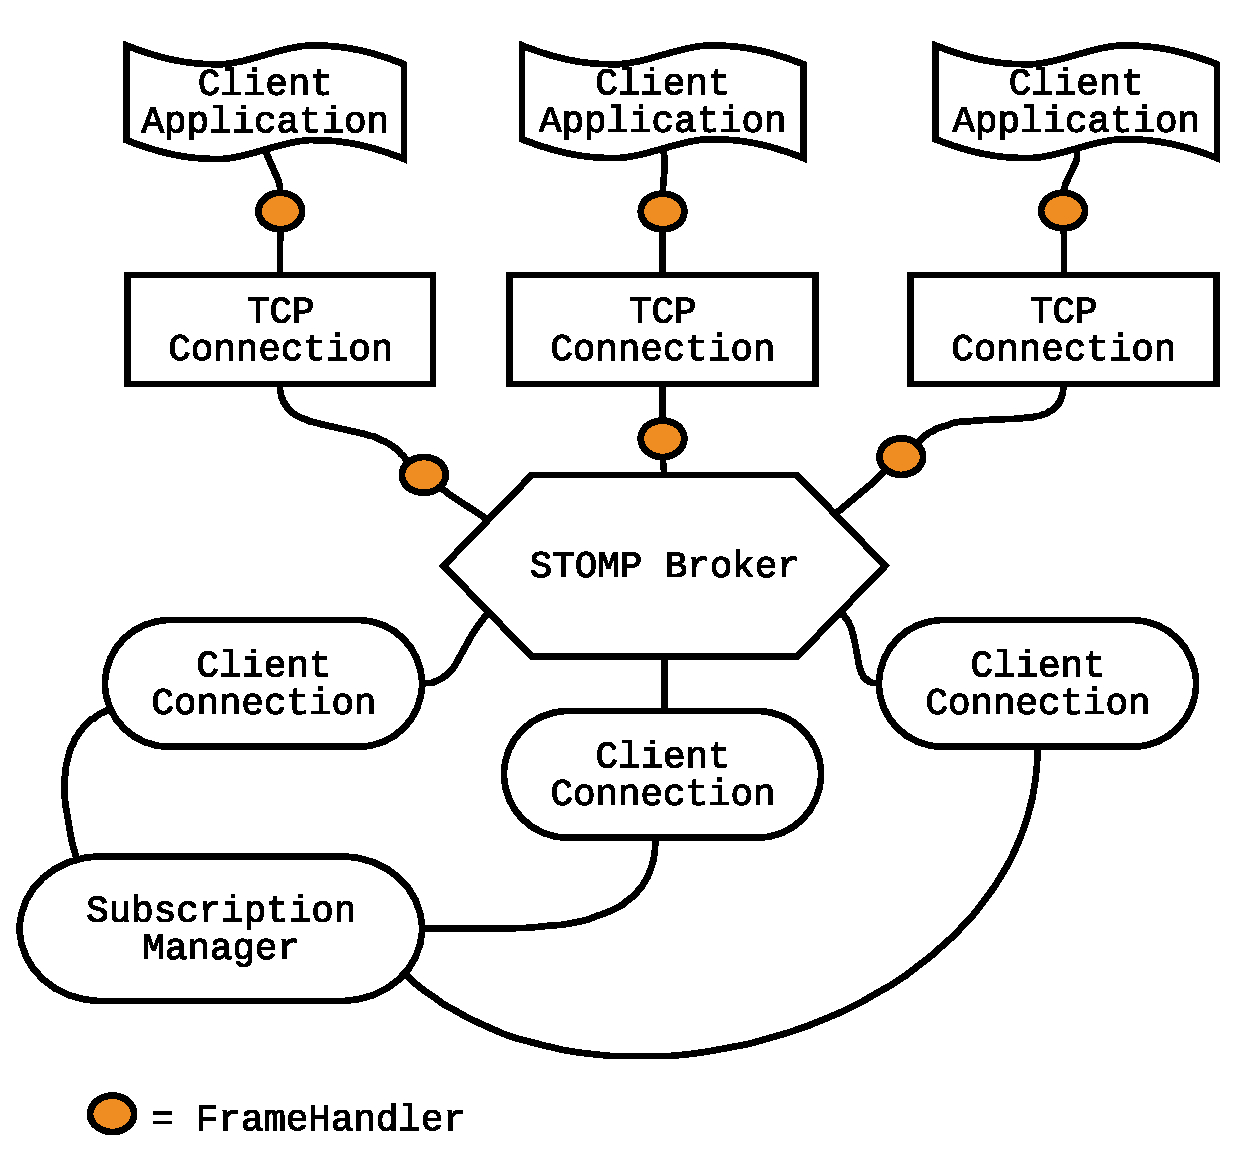
\includegraphics[scale=.30]{architecture.pdf}
        \caption{STOMP Broker Architecture}
    \end{figure}
\else
\fi

The server itself maintains a separate stateful loop in the \textit{SubscriptionManager}. The \textit{SubscriptionManager} is a per-broker singleton that manages all of the subscriptions for all of the clients across that server. As clients subscribe to destinations, the \textit{SubscriptionManager} is updated with that information.

\subsection{The Subscriptions Module}

The \textit{Subscriptions} module exports a \textit{SubscriptionManager} that client threads use to report updates to client subscriptions. Subscription handling is the most complex portion of the system. Initialization of the \textit{SubscriptionManager} involves forking off two separate stateful loops: one to maintain the state of active client subscriptions, and one to maintain the state of message acknowledgements.

\ifCLASSINFOpdf
    \begin{figure}[h]
        \centering
        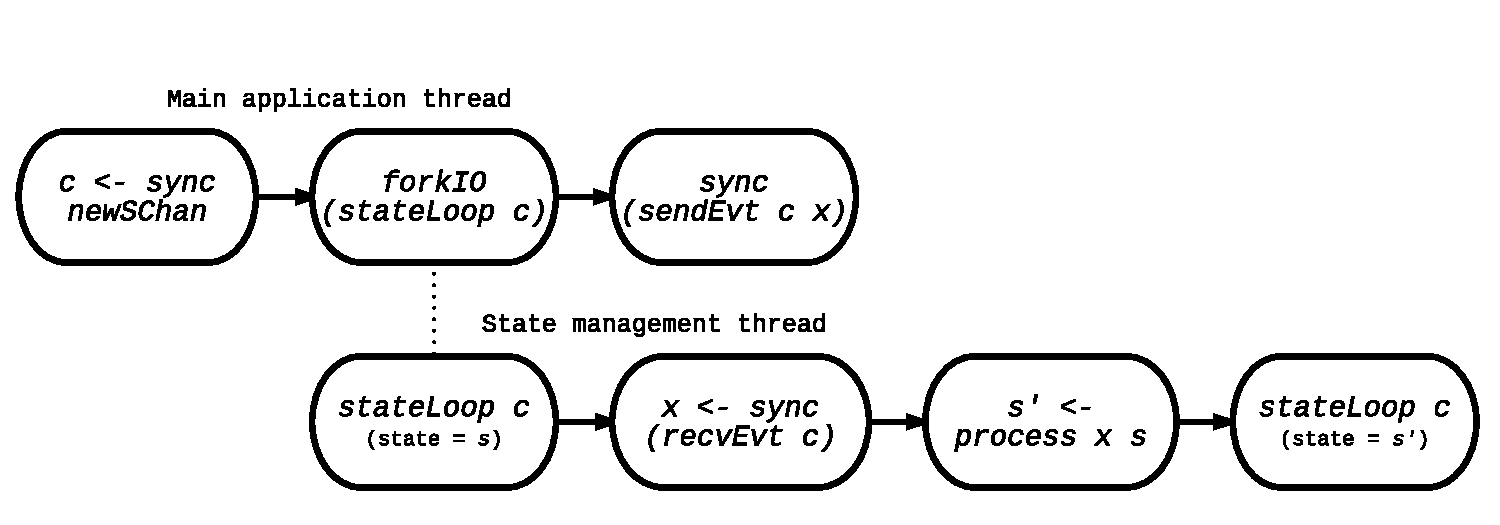
\includegraphics[scale=.30]{state_management.pdf}
        \caption{State Management Workflow}
    \end{figure}
\else
\fi

\begin{figure}[h]
    \begin{minted} {haskell}
    type ClientId            = Integer
    type SubscriptionId      = String

    type SubMap = HashMap 
      Destination (HashMap ClientId ClientSub)

    type ClientDests = HashMap 
      ClientId (HashMap SubscriptionId Destination)

    data Subscriptions = Subscriptions SubMap ClientDests

    -- |Initialize a SubscriptionManager and return it in 
    -- an IO context.
    initManager :: IO SubscriptionManager
    initManager = do
        updateChan <- sync newSChan
        ackChan    <- sync newSChan
        inc        <- newIncrementer
        subs       <- return $ Subscriptions HM.empty HM.empty
        forkIO $ updateLoop updateChan ackChan subs inc
        forkIO $ ackLoop ackChan updateChan HM.empty
        return $ SubscriptionManager updateChan
    \end{minted}
    \centering
    \caption{Forking State Loops in the SubscriptionManager}
\end{figure}

The \textit{Subscriptions} datatype houses the state that needs to be maintained in the \textit{updateLoop} function. It contains a \textit{SubMap}, which maps destinations to collections of client subscriptions. It also contains a datatype called \textit{ClientDests}. This is not strictly necessary, and makes for a somewhat more complex implementation, but there is a desirable tradeoff in efficiency for unsubscribe operations. The \textit{ClientDests} contains mappings of \textit{ClientId} and \textit{SubscriptionId} pairs to \textit{Destinations}. This is to enable fast unsubscribe operations:  \textit{O(log(n))} compared to \textit{O(d)}, where \textit{n} is the number of clients and \textit{d} is the number of active destinations. Using these two datastructures in conjunction, though somewhat complicated, precludes the need to search through all destinations to see if they countain the given mapping.

The state of \textit{Subscriptions} is managed by abstracting all subscription operations through event-generating functions that send updates on the \textit{updateChan}. As SUBSCRIBE, UNSUBSCRIBE, and SEND frames are received, the client thread calls the appropriate update function and the \textit{updateLoop} adjusts the state of the data accordingly as part of processing the update. This is a broadly useful pattern when developing concurrent applications, as most useful programs need some way of maintaining running state in various components, and it is made exceptionally straightforward using transactional events.

\begin{figure}[h!]
    \begin{minted} {haskell}
    -- |General Update type for main processing loop
    data Update = 
      Add Destination ClientSub |
      Remove ClientId SubscriptionId |
      GotMessage Destination Frame |
      ResendMessage Destination Frame [ClientId] MessageId |
      Ack ClientAckResponse |
      Disconnected ClientId

    -- |State management loop for Subscriptions
    updateLoop :: 
      SChan Update ->
      Subscriptions -> 
      IO ()
    updateLoop updateChan subs = do
        update <- sync $ recvEvt updateChan
        subs'  <- handleUpdate update subs
        updateLoop updateChan subs'

    -- |Send a Frame to a Destination 
    -- (example of an exported update function)
    sendMessageEvt :: 
      SubscriptionManager -> 
      Destination -> 
      Frame -> 
      Evt ()
    sendMessageEvt 
      manager@(SubscriptionManager updateChan) 
      destination 
      frame = 
        sendEvt updateChan $ GotMessage destination frame
    \end{minted}
    \centering
    \caption{State Management for Subscriptions}
    \label{statemanagecode}
\end{figure}


The code in Figure \ref{statemanagecode} is a slight simplification of the update code in the \textit{Subscriptions} module (some parameters are left out for space considerations), but it is illustrative of how transactional events easily enable this pattern. It's incredibly straightforward to reason about and build such state management loops without the overhead of a heavyweight framework or convoluted imperative-style logic. The entire operation of maintaining state is abstracted into three basic operations: (1) wait for an update, (2) process the update  (3) return a modified state from the update processing. We have a loop that waits for updates on its synchronous channel. When one is received, it is processed by a function that returns a (potentially) modified subscription mapping. We then proceed to the next loop iteration with the updated state.

\subsection{Client Selection in Message Processing}

The distributed model enabled by the STOMP broker is that of a many clients acting as both producers and consumers. An individual message is produced by one client and consumed by another. There are other possible implementation-specific behaviors (such as one-to-many broadcast) that are not strictly dictated by the protocol, but those have not been implemented for this project. One client produces a message and delivers it to a destination; some other client, acting as a consumer, subscribes to a destination, advertising its willingness to process messages sent to that destination. As there could potentially be multiple clients subscribed to a single destination, the broker needs some mechanism by which to choose the ``most eligible" client for consumption of a given message. We can imagine several possible approaches to this problem. We could choose a client at random, but we run the risk of that client being blocked on some other operation. We could implement a "round-robin" approach, where every client gets a turn, but we run into the same risk; the chosen client might be blocked. One could imagine some sort of complicated suitability heuristic, but what would that logic even look like? Transactional events can make this choice straightforward to implement using the non-deterministic \textit{chooseEvt} combinator. Events can be constructed dynamically from a map containing client channels. When we synchronize on the event, the first client thread that is able to complete the transaction will do so, with all other events fizzling without having sent the message to their respective clients.

\begin{figure}[h]
\begin{minted} {haskell}
clientChoiceEvt :: 
  Frame -> 
  MessageId -> 
  [ClientId] -> 
  HashMap ClientId ClientSub -> 
  Evt (Maybe ClientSub)
clientChoiceEvt frame messageId sentClients = 
    HM.foldr 
        (partialClientChoiceEvt frame messageId sentClients) 
          $ (timeOutEvt 500000) 
              `thenEvt` (\_ -> alwaysEvt Nothing)

partialClientChoiceEvt :: 
  Frame -> 
  MessageId -> 
  [ClientId] -> 
  ClientSub -> 
  Evt (Maybe ClientSub) -> 
  Evt (Maybe ClientSub)
partialClientChoiceEvt 
  frame 
  messageId 
  sentClients 
  sub@(ClientSub clientId _ _ frameHandler) = 
    if clientId `elem` sentClients then 
        (chooseEvt neverEvt) 
    else let frame' = transformFrame frame messageId sub in
        chooseEvt $ 
            (putEvt frame' frameHandler) 
                `thenEvt` (\_ -> alwaysEvt $ Just sub)
\end{minted}
\centering
\caption{Nondeterministic Choice of Consumer}
\end{figure}

The above code demonstrates the dynamic event construction for client choice. There are a few implementations details to take note of here. First, notice that the event is constructed using a recursive fold over the map of client subscriptions. The base case in the fold is a \textit{timeOutEvt} that returns \textit{Nothing} after a half second's wait. If there are no clients available to synchronize on the message within a half second, we retry the send, as it is possible that new subscribers have been registered in that time. If \textit{Nothing} is returned from this event, we simply fork off an update to the main processing loop. Also, notice the \textit{sentClients} list; this list contains all those client identifiers of clients to whom the message was sent and subsequently NACK'd (disacknowledged). We do not want to continually send a message to a client that has already rejected the message, so we maintain a running list in the \textit{AckContext} and use it here to avoid doing so.
\subsection{The Transaction Module}

The \textit{Transaction} module exports a \textit{ClientTransactionManager} to each client thread that is used to report updates to client transactions. It uses the same state management pattern described in the section on the \textit{Subscriptions} module to maintain what could potentially be multiple ongoing transactions for a single client. When a BEGIN frame is received, a transaction is initiated. We do so by inserting a unit \textit{alwaysEvt} into the mapping. As additional frames are received, the transactional event is constructed dynamically using the \textit{thenEvt} combinator. This ensures that when we synchronize on the final event, all component events occur in sequence. This also ensures that all component events synchronize in sequence \textit{atomically}, an important guarantee. They are not processed by the \textit{SubscriptionManager} asynchronously; no other events are processed until all events in the transaction composite are processed sequentially. Such a composite event, in which two messages are sent as part of a transaction, would look something like this:

\begin{figure}[h]
\begin{minted} {haskell}
alwaysEvt ()
    `thenEvt` ((\_ -> sendMessageEvt subManager d1 f1)
        (`thenEvt` (\_ -> sendMessageEvt subManager d2 f2)))
\end{minted}
\centering
\caption{Composite Transactional Event For a STOMP Transaction}
\label{compositevt}
\end{figure}

There is something subtle in the construction of this event that may not be immediately apparent. In order for this event to synchronize, the \textit{SubscriptionManager} must support the ability to receive multiple updates in one synchronization. Recall the implementation of the \textit{updateLoop} function in the section detailing the \textit{SubscriptionManager}. Given that implementation, only one update is possible per event synchronization. As such, our event will compile, but will block indefinitely on synchronization, as the server will be waiting for the first update syncrhonization to complete prior to looping through and accepting the next update. The addition of transaction handling hence required an update to the \textit{SubscriptionManager} to support such updates. Kehrt, Effinger-Dean, Schmitz, and Grossman identify this particular issue in \cite{te:idioms}, and their solution pattern is applied here successfully. We make the following change to the \textit{updateLoop} function in the \textit{Subscriptions} module (once again the code, in particular the number of parameters, is slightly simplified for purposes of demonstration):

\begin{figure}[h]
\begin{minted} {haskell}
-- |State management loop for Subscriptions
updateLoop :: 
  SChan Update -> 
  SChan AckUpdate -> 
  Subscriptions -> 
  IO ()
updateLoop updateChan subs = do
    subs' <- sync $ updateEvtLoop updateChan subs
    updateLoop updateChan subs'

-- |Looping event to handle the possiblility of
-- multiple subsequent transactional synchronizations 
-- in the updateLoop
updateEvtLoop :: 
  SChan Update -> 
  Subscriptions -> 
  Evt Subscriptions
updateEvtLoop updateChan subs = do
    update <- recvEvt updateChan
    subs'  <- handleUpdate update subs updateChan
    (alwaysEvt subs') `chooseEvt` 
        (updateEvtLoop updateChan subs')
\end{minted}
\centering
\caption{Looping Transactional Event}
\end{figure}

Instead of synchronizing on a single update and then using that to update the state of the subscriptions, we create a composite event that has the ability to synchronize on arbitrarily many sequential updates, returning updated subscriptions with each iteration. We achieve this through use of the sequencing monadic bind (recall that this uses the \textit{thenEvt} combinator) and the \textit{chooseEvt} combinator. The event must first receive an update on the channel, then handle the update, and then either receive another update or complete and return the updated \textit{Subscriptions}. One might, upon first glance, wonder whether this functions as we would expect due to the non-deterministic nature of the \textit{chooseEvt} combinator. However, since we are sequencing the event using Haskell's \textit{do} notation, every event in the sequence must be able to complete. If the initiating event were a sequence of sends on the \textit{updateChan}, the composite would not be able to complete if the \textit{alwaysEvt} were chosen, so the semantics of transactional events dictates that the \textit{updateEvtLoop} choice \textit{must} be taken until there are no more sends that need to be matched, at which point the \textit{alwaysEvt} will be chosen and the final result returned.

\section{Client Application Design \& Usage}

The STOMP client implemented for this project is a basic command-line client. It is not particularly representative of ``real-world" usage of a STOMP client, but is rather intended for interactive demonstration of the capbabilities of the message broker.

The approach to the client design is ``event-driven". There are multiple asynchronous state loops that send events to the main session loop, which handles them synchronously.

\subsection{Client Commands}

A listing and description of client commands in this application is given.

\begin{itemize}
    \item \textbf{connect [hostname] [port]}: connect to a STOMP broker on the given hostname/port combination.
    \item \textbf{disconnect}: disconnect from an active session
    \item \textbf{send [destination] [message]}: Send a text frame containing the given message to the given destination.
    \item \textbf{sendr [destination] [receipt-id] [message]}: Send a text frame containig the given message to the given destination. Request a receipt with the given receipt-id.
    \item \textbf{loopsend [n] [destination] [message]}: Send a text frame containing the given message to the given destination n times in a row.
    \item \textbf{subscribe [destination]}: Subscribe to the given destination.
    \item \textbf{unsubscribe [subscription-id]}: Unsubscribe from the subscription with the given subscription id.
    \item \textbf{begin [tx-id]}: Begin a named transaction with the tx-id as the transaction identifier. All send and sendr commands prior to either a commit or an abort will be send as part of this transaction.
    \item \textbf{commit}: Commit the transaction in process, if such exists.
    \item \textbf{abort}: Abort the transaction in process, if such exists.
    \item \textbf{subs}: List details about all active subscriptions
    \item \textbf{exit}: Close the active session (if any) and exit the application.
\end{itemize}
\section{Conclusions}

We have shown that a fairly large and complex concurrent application can be successfully built using transactional events as a foundation for inter-process communications and library design. Additionally, we have used transactional events to their full effect in leveraging their guarantee of atomicity when committing client transactions in our message broker application. We have also identified many additional useful patterns that stem from using a message-passing abstraction. The authors of \cite{te:original} state that the abstraction provides greater modularity and eases reasoning about concurrent programs, and, while that may indeed be subjective and difficult to quantify, we believe that the work accomplished here validates that claim. Indeed, it is fairly clear that the solutions given here would have been extremely complex and bug-prone, if not outright impossible, were they to have been implemented given some other concurrency model.

\section{Related Work}
To date there has been relatively little work around transactional events aside from the foundational work done by
Fluet and Donnelly in 2008 \cite{te:original}. Fluet and Amsden extend this foundation with a refined semantics  for ``fairness" in 2011 \cite{te:fairness}.
A detailed account of a large-scale implementation utilizing the abstraction does not appear to exist in the literature. 
In addition to Haskell, the semantics outlined in Fluet and Donnelly's 2008 work have been implemented in ML \cite{te:ml}. 
Kehrt, Effinger-Dean, Schmitz, and Grossman identify some basic problems that arise from some simple use cases for
transactional events, and propose idiomatic approaches to these issues in their work ``Programming Idioms for Transactional Events" \cite{te:idioms}.  

\bibliographystyle{IEEEtran}
\bibliography{IEEEabrv,citations}

\clearpage
\begin{appendices}

\section{Module Dependencies for tehstomp-lib}

\ifCLASSINFOpdf
    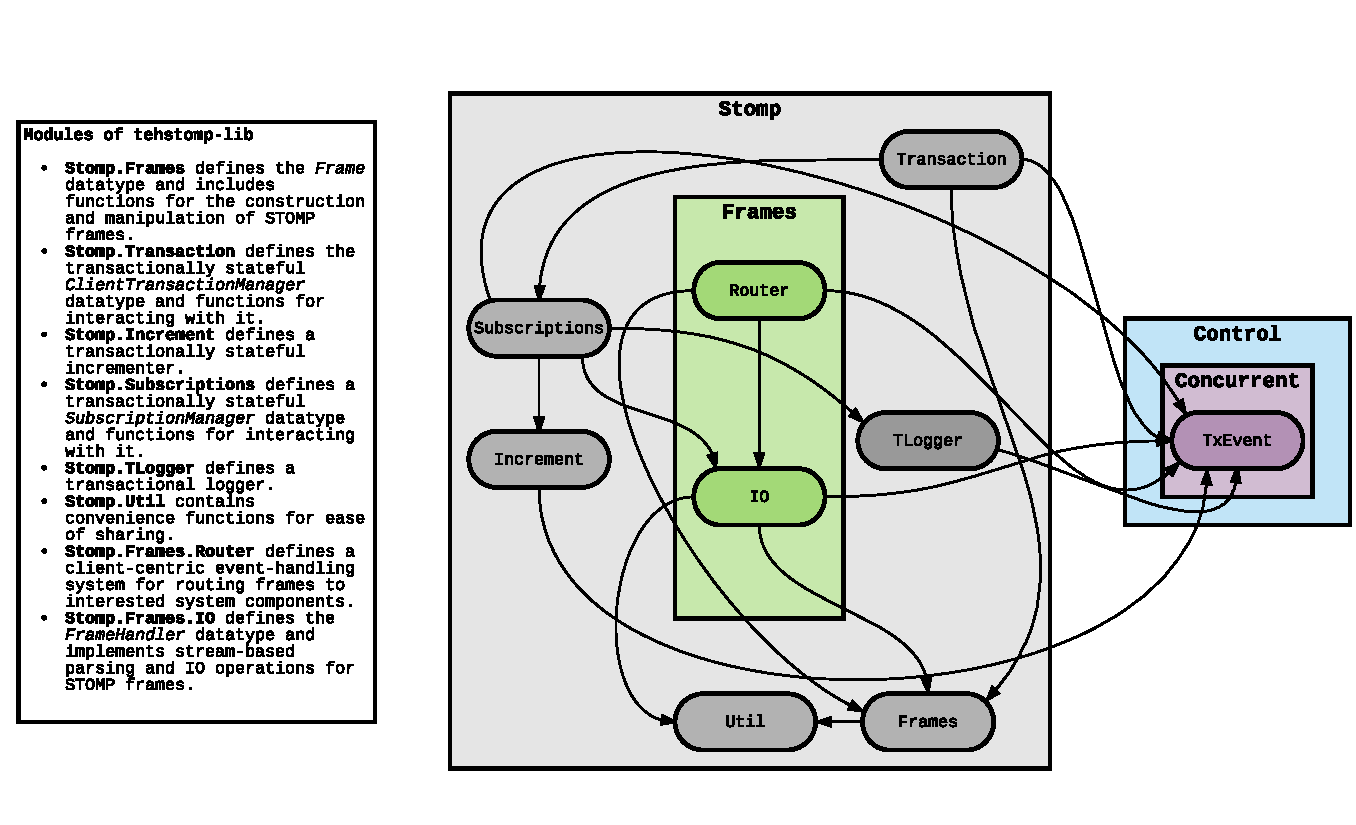
\includegraphics[scale=.8]{dependencies.pdf}
\else
\fi

\end{appendices}

\end{document}
